\documentclass[12pt]{article}
\usepackage[utf8]{inputenc} % uft8 you know
\usepackage[danish]{babel}
\usepackage{lastpage}
\usepackage{fancyhdr}
\usepackage{hyperref}
\usepackage{comment}
\usepackage[
backend=biber,
style=apa,
sorting=ynt
]{biblatex}
\addbibresource{sources/library.bib}
\usepackage[T1]{fontenc}
\usepackage{ae}
\usepackage{graphicx}
\usepackage{array}
\usepackage{ragged2e} % for \RaggedRight command
\usepackage{booktabs} % for \toprule, \midrule, \bottomrule
\usepackage{pdfpages} % Til at inkludere pdf'er
\usepackage{amsmath}
\usepackage{amsfonts}
\usepackage{amssymb}
\usepackage{longtable}
\usepackage{adjustbox}
\usepackage{blindtext}
\usepackage{geometry}
\usepackage{multirow}
%\usepackage{natbib} % Works with.bib files
%\bibliographystyle{apalike} 
\usepackage{tabularx, booktabs, siunitx} % From now on ist only code styling!
% Default fixed font does not support bold face
\DeclareFixedFont{\ttb}{T1}{txtt}{bx}{n}{12} % for bold
\DeclareFixedFont{\ttm}{T1}{txtt}{m}{n}{12}  % for normal
% Custom colors
\usepackage{color}
\definecolor{deepblue}{rgb}{0,0,0.5}
\definecolor{deepred}{rgb}{0.6,0,0}
\definecolor{deepgreen}{rgb}{0,0.5,0}
\newcommand\pythonstyle{\lstset{
language=Python,
basicstyle=\ttm,
morekeywords={self},              % Add keywords here
keywordstyle=\ttb\color{deepblue},
emph={MyClass,__init__},          % Custom highlighting
emphstyle=\ttb\color{deepred},    % Custom highlighting style
stringstyle=\color{deepgreen},
frame=tb,                         % Any extra options here
showstringspaces=false,
breaklines=true
}}

\usepackage{hyperref}
\usepackage{caption}
\DeclareCaptionFont{white}{\color{white}}
\DeclareCaptionFormat{listing}{\colorbox{blue}{\parbox{\textwidth}{\hspace{15pt}#1#2#3}}}
\captionsetup[lstlisting]{format=listing,labelfont=white,textfont=white, singlelinecheck=false, margin=0pt, font={bf,footnotesize}}
\usepackage{listings}

\geometry{
    a4paper,
    total={170mm,257mm},
    left=20mm,
    top=30mm,
    bottom=30mm,
}
\hypersetup{
    linkcolor=black,
    colorlinks=false,
    pdftitle={SOP - Kristoffer Frøkjær Sørensen},
    pdfauthor={Kristoffer Frøkjær Sørensen},
    % Remove the red border around links
    pdfborder={0 0 0},
}

\pagestyle{fancy} % definds the pagestyleing
\fancyhf{} % Removes the wired header text
\renewcommand{\headrulewidth}{0pt} % Removes the line under the header
\cfoot{Side \thepage\ af \pageref{LastPage}} % Sets the right side of the footer to "Page X of Y"
%\lhead{Gruppe 1} % Sets the left side of the header to "Gruppe 1"

\begin{document}
    % Python environment
    \lstnewenvironment{python}[1][]
    {
    \pythonstyle
    \lstset{#1}
    }
    {}
    % Python for external files
    \newcommand\pythonexternal[2][]{{
    \pythonstyle
    \lstinputlisting[#1]{#2}}}
    % Python for inline
    \newcommand\pythoninline[1]{{\pythonstyle\lstinline!#1!}}

    \lstnewenvironment{JavaScript}[3][]
    {
    \JavaScriptStyle
    \lstset{#2}
    }
    {}

    \lstloadlanguages{C,C++,csh,Java}

\definecolor{red}{rgb}{0.6,0,0} 
\definecolor{blue}{rgb}{0,0,0.6}
\definecolor{green}{rgb}{0,0.8,0}
\definecolor{cyan}{rgb}{0.0,0.6,0.6}

\lstset{
language=csh,
basicstyle=\footnotesize\ttfamily,
numbers=left,
numberstyle=\tiny,
numbersep=5pt,
tabsize=2,
extendedchars=true,
breaklines=true,
frame=b,
stringstyle=\color{blue}\ttfamily,
showspaces=false,
showtabs=false,
xleftmargin=17pt,
framexleftmargin=17pt,
framexrightmargin=5pt,
framexbottommargin=4pt,
commentstyle=\color{green},
morecomment=[l]{//}, %use comment-line-style!
morecomment=[s]{/*}{*/}, %for multiline comments
showstringspaces=false,
morekeywords={ abstract, event, new, struct,
as, explicit, null, switch,
base, extern, object, this,
bool, false, operator, throw,
break, finally, out, true,
byte, fixed, override, try,
case, float, params, typeof,
catch, for, private, uint,
char, foreach, protected, ulong,
checked, goto, public, unchecked,
class, if, readonly, unsafe,
const, implicit, ref, ushort,
continue, in, return, using,
decimal, int, sbyte, virtual,
default, interface, sealed, volatile,
delegate, internal, short, void,
do, is, sizeof, while,
double, lock, stackalloc,
else, long, static,
enum, namespace, string},
keywordstyle=\color{cyan},
identifierstyle=\color{red}
}

    %\providecommand\NAT
    \title{
    SOP - Mindste kvadraters metode \\ 
    \large{Rybners HTX - Vejleder: Carsten Finn Sørensen og Vicki Jacob} \\
    \small{Programering B og Matematik A}
}
\author{Af Kristoffer Sørensen}
\thispagestyle{empty}
\maketitle
%\begin{figure}[h!]
  %  \centering
  %  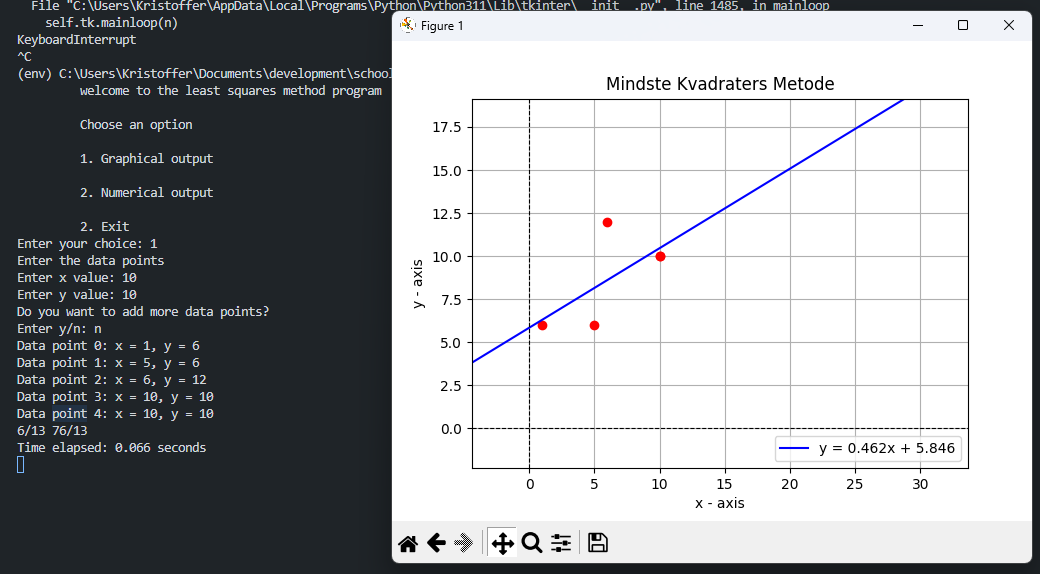
\includegraphics[width=0.9\textwidth]{figurs/forsideimg.jpg}
  %  \caption{Nuclear Bomb Explosion - Mushroom Cloud stock photo (\cite{RomoloTavani2018}) }%\cite{Forsideimg}} TODO: Add source
 %   \label{fig:Forsideimg}
%\end{figure}
\newpage
    \newpage
    %\bibliography{sources/library}\printbibliography
    \printbibliography[ heading=bibintoc, title={Litteratur}]
    \newpage

\section{Bilag}\label{sec:Bilag}
\subsection{Bilag 1: Koden}\label{sec:koden}
\begin{python}
    from sympy import symbols, solve, Eq, diff
import matplotlib.pyplot as plt
import numpy as np 
import time

def leastSquaresMethod(dataPoints):
    startTime = time.time() # Gets the current time
    a, b = symbols('a b')
    sumA2 = 0 # Sum of a^2 
    sumB2 = 0 # Sum of b^2
    sumAB = 0 # Sum of 2ab
    sumA = 0 # Sum of 2ax
    sumB = 0 # Sum of 2by
    sumConstant = 0
    n = len(dataPoints) # Gets the number of data points

    for i in range(n): # Loops through all data points and calculates the sums
        x = dataPoints[i][0] # Gets the x value of the data point
        y = dataPoints[i][1] # Gets the y value of the data point
        print(f"Data point {i}: x = {x}, y = {y}") # Prints what data point is being calculated
        sumA2 += a**2 * x**2 # Adds the sum of a^2
        sumB2 += b**2      # Adds the sum of b^2
        sumAB += 2*a*b*x   # Adds the sum of 2ab
        sumA += 2*a*x*y   # Adds the sum of 2ax
        sumB += 2*b*y    # Adds the sum of 2by
        sumConstant += 2*y # Adds the sum of 2c

    # Defines the function of two variabel containing the sum of squared errors
    f = sumA2 + sumB2 + sumAB - sumA - sumB + sumConstant 

    # Solve for a and b
    diffA = diff(f, a) # Differentiates f to a
    diffB = diff(f, b) # Differentiates f to b
    solutions = solve([diffA, diffB], (a, b)) # Solves the equations
    print(solutions[a], solutions[b]) # Prints the solutions
    timeElapsed = time.time() - startTime # Calculates the time elapsed
    print(f"Time elapsed: {timeElapsed:.3f} seconds") # Prints the time elapsed
    return solutions[a], solutions[b] # Returns the solutions as a tuple containing a and b [a, b]

def plotter(dataPoints):
    line = leastSquaresMethod(dataPoints) # Calls the leastSquaresMethod function and stores the result in line
    slope = float(line[0])  # Gets the slope of the line
    intercept = float(line[1])  # Gets the intercept of the line
    
    for point in dataPoints: # Loops through all data points and plots them
        plt.plot(point[0], point[1], 'ro')
    
    # Defince x values for the line
    x = np.linspace(-10, 100, 100)  # Creates a interval of the line. The line will be drawn from -10 to 100
    y = slope * x + intercept # Calculates the y values for the line
    
    # Plot linjen
    plt.plot(x, y, label=f"y = {slope:.3f}x + {intercept:.3f}", color='blue') # Plots the line
    plt.quiver(x[0], y[0], -1, -slope, angles='xy', scale_units='xy', scale=1, color='blue', width=0.003) # Adds an arrow to the start of the line
    plt.quiver(x[-1], y[-1], 1, slope, angles='xy', scale_units='xy', scale=1, color='blue', width=0.003) # Adds an arrow to the end of the line
    
    # Akse og grid
    plt.axhline(0, color='black', linewidth=0.8, linestyle='--') # Adds a horizontal line at y = 0
    plt.axvline(0, color='black', linewidth=0.8, linestyle='--') # Adds a vertical line at x = 0
    plt.title('Mindste Kvadraters Metode') # Adds a title to the plot
    plt.xlabel('x - axis') # Adds a label to the x-axis
    plt.ylabel('y - axis') # Adds a label to the y-axis
    plt.legend() # Adds a legend to the plot
    plt.grid() # Adds a grid to the plot
    plt.show() # Shows the plot

def main():
    print("\t welcome to the least squares method program")
    print("\n \t Choose an option")
    print("\n \t 1. Graphical output")
    print("\n \t 2. Numerical output")
    print("\n \t 2. Exit")
    userInput = input("Enter your choice: ")
    if userInput == "1":
        print("Enter the data points")
        dataPoints = [(1, 6), (5, 6), (6, 12), (10,10)]
        while True:
            x = input("Enter x value: ")
            y = input("Enter y value: ")
            dataPoints.append((int(x), int(y)))
            print("Do you want to add more data points?")
            choice = input("Enter y/n: ")
            if choice == "n":
                break
        plotter(dataPoints)
        main()
    elif userInput == "2":
        while True:
            x = input("Enter x value: ")
            y = input("Enter y value: ")
            dataPoints.append((int(x), int(y)))
            print("Do you want to add more data points?")
            choice = input("Enter y/n: ")
            if choice == "n":
                break
        plotter(dataPoints)
        main()
    elif userInput == "3":
        exit()
    else:
        print("Invalid input")
        main()

main()
\end{python}
\end{document}